\section{\method}
\subsection{装置と用語解説}
この実験にはMathWorks\raisebox{2mm}{\tiny\textregistered}社の\matlab を用いて,\tblref{tbl:実験環境}の環境下で実験する.
\begin{table}[H]
    \caption{実験環境}
    \label{tbl:実験環境}
    \begin{tabularx}{\columnwidth}{cR}
        \hline
        \multirow{2}{*}{実験機}   & MacBook Air 2022 (Apple社)   \\
                               & 型番:\texttt{MLY13J/A}        \\
        \hline
        \multirow{2}{*}{プロセッサ} & Apple Silicon M2            \\
                               & 8コアCPU,8コアGPU               \\
        \hline
        メモリ                    & 8GB                         \\
        \hline
        ブラウザ                   & Safari\ バージョン16.5           \\
        \hline
        ImageJ                 & 1.53k\ Java 13.0.6 (64-bit) \\
        \hline
    \end{tabularx}
\end{table}
\paragraph{HTML}
Hyper Text Markup Languageの略で,Webページを作成するためのマークアップ言語.Webページ上のテキストデータに「タグ」を与えて,文字の大きさ,色やフォントを変更する.
\paragraph{CSS}
Cascading Style Sheetsの略で,Webページのスタイルを指定するための言語である.CSSの適用により,ホームページの文字や背景などがタグを利用して統一される.
\paragraph{JavaScript}
ブラウザ上で動作するアプリケーションを記述するための言語である.現在のWebアプリケーション上でデファクトスタンダード言語である\cite[p.68]{CGとゲームの技術}.
\subsection{JavaScriptの初歩}
\begin{itemize}
    \item \textbf{\texttt{A.indexOf("Strings")}}\\
          JavaScriptには,\texttt{A.indexOf("Strings")}で,\texttt{Strings}が\texttt{A}に含まれていることを確認できる.含まれていない場合は,\texttt{-1}を戻り値とし,含まれている場合はその箇所を自然数で返す.
    \item \textbf{User Agent(UA)}\\
          User Agent(UA)とは,利用者のブラウザとOSを指す.
          この実験で利用するUAは,macOSのSafariである.
          SafariにはUAを変更する機能がある.Chrome,Firefox,MicrosoftEdge,Safari 16.4は,SafariのUA切り替え機能を用いて実験する.
\end{itemize}
\kadai{ブラウザ判定}\par
\texttt{Navigator object}オブジェクトの\texttt{userAgent}プロパティを用いて,利用ブラウザを判定する.
\texttt{A}に\texttt{Strings}が含まれていない場合,戻り値は\texttt{-1}である.この実験では,ブラウザがFirefoxである場合は\ \texttt{this browser is Firefox}\ ,そうでない場合は\ \texttt{this browser is not Firefox}\ と表示するWebページを作成する.\\
\kadai{ブラウザによるCSSの切り替え}\par
ブラウザ判定を用いて,ブラウザによってCSSを変更するJavaScriptを記述する.CSSを設定する\texttt{link}タグに\texttt{id}を指定し,\texttt{document.getElementById}関数で\texttt{link}タグをインスタンス化する.
ブラウザ判定結果により,このインスタンスを利用してCSSを変更する.この実験では,CSSで背景色のみを変更する.UAと指定背景色は\tblref{tbl:UAと指定背景色}に示す.
\begin{table}[H]
    \centering
    \caption{UAと指定背景色}
    \label{tbl:UAと指定背景色}
    \begin{tabularx}{\columnwidth}{RRR}
        \multicolumn{1}{c}{UA} & \multicolumn{1}{c}{背景色}    & \multicolumn{1}{c}{CSS名} \\
        \hline
        Firefox                & \rulebox{{orange}}{orange} & \texttt{firefox.css}     \\
        Chrome                 & \rulebox{{blue}}{blue}     & \texttt{chrome.css}      \\
        Other                  & \rulebox{{gray}}{gray}     & \texttt{default.css}     \\
        \hline
    \end{tabularx}
\end{table}
ここで,MicrosoftEdgeは,UAに\texttt{"Chrome"}文字列と\texttt{"Edge"}文字列を持つ.正確に\texttt{Chrome}を判別するには,条件式に,「\texttt{"Chrome"}を含み\texttt{"Edge"}を除く」処理を記述する必要がある.\\
\kadai{時刻によるCSSの切り替え}\par
JavaScriptで現在時刻を取得するには,\texttt{Date}をインスタンス化する必要がある.\texttt{Date}内の\texttt{getSeconds}関数を呼び出すことで,現在時刻の「秒」を得られる.
この実験では,現在時刻\footnote{正確には,HTMLを読み込んだ時刻.}の秒数を\(n\)とすると,以下の条件でCSSを変更する.
\begin{equation*}
    \textrm{適用するCSS}=
    \begin{cases}
        \texttt{firefox.css} & (0\leq n<20)  \\
        \texttt{chrome.css}  & (20\leq n<40) \\
        \texttt{default.css} & (40\leq n<60)
    \end{cases}
\end{equation*}
\kadai{マウスイベントの取得}\par
この実験では,「現在時刻の取得」と書かれた文字上をクリックすると,クリックした時刻をリストとして後ろに追加するプログラムを記述する.文字列「現在時刻の取得」をひとつのオブジェクトとして定義するため,\texttt{<span></span>}タグを用いる.
また,リストアイテムとして表示するために,現在時刻を\texttt{<ul></ul>}タグ内の要素\texttt{<li></li>}タグへ格納する.\par
\begin{enumerate}
    \item 「現在時刻の取得」文字列を\texttt{<p></p>}タグの属性\texttt{onmousedown}で,現在時刻をリストアイテムとして追加する関数\texttt{input\_item()}を呼び出す.この関数を呼び出すと,変数\texttt{time}に,時刻\texttt{Hour:Minutes:Second}が格納される.
    \item \texttt{<ul></ul>}に対して,\texttt{document.getElementById}関数を用いてインスタンス名\texttt{list}でインスタンス化する.
    \item \texttt{document.createElement("li")}関数を用いて,\texttt{<li></li>}タグを生成し,変数\texttt{listItem}に格納する.
    \item \texttt{listItem}の要素を\texttt{listItem.textContent}で指定し,\texttt{time}を代入する.
    \item \texttt{list.appendChild(listItem)}で\texttt{listitem}を子要素として組み込む.
\end{enumerate}
\subsection{色覚}
色覚は,光の刺激により色を見分ける感覚である\cite{2020新明解国語辞典}.
すべての色は,光の三原色と呼ばれる「赤」「緑」「青」から構成される.
色を感じとる視細胞も,赤緑青それぞれに敏感な細胞が3種類存在する.
色覚異常はこの3種類の視細胞のうちどれか足りなかったり,十分に機能しないために起こる\cite{色覚の異常}.
各色覚の見え方を\tblref{tbl:各色覚の見え方}に示す.
\begin{figure}[H]
    \centering
    \begin{tikzpicture}
        \draw[thick,-latex](-.3,0)--(6.5,0)node[midway,below=.4cm]{\small 光の波長(nm)};
        \draw[thick,-latex](-.3,0)--(-.3,3)node[midway,left]{\small \rotatebox{90}{光に対する感度}};
        \foreach \u \v in {0/400,1/450,2/500,3/550,4/600,5/650,6/700}
        \draw(\u,-0.1)node[below]{\scriptsize \v}--(\u,0);
        \foreach \u in {0,0.2,...,6}
        \draw(\u,0)--(\u,0.1);
        \foreach \u in {0.3,0.6,...,3.0}
        \draw(-.3,\u)--(-.2,\u);
        \draw[very thick,blue,dotted]plot[smooth,tension=0.7]coordinates{(0,1.8)(0.8,2.7)(2.8,0.6)(4.8,0)};
        \draw[very thick,green!50!gray,dashed]plot[smooth,tension=0.7]coordinates{(0,0.6)(0.4,1.2)(0.8,1.5)(2.8,2.7)(5.6,0.3)};
        \draw[very thick,red,densely dash dot dot]plot[smooth,tension=0.7]coordinates{(0,0.6)(0.4,1.2)(1,1.45)(3.2,2.8)(6,0.6)};
    \end{tikzpicture}
    \begin{tikzpicture}
        \draw[very thick,blue,dotted](0,0)--(2,0)node[right,color=black]{青に敏感な視細胞(S錐体)};
        \draw[very thick,green!50!gray,dashed](0,-.5)--(2,-.5)node[right,color=black]{緑に敏感な視細胞(M錐体)};
        \draw[very thick,red,densely dash dot dot](0,-1)--(2,-1)node[right,color=black]{赤に敏感な視細胞(L錐体)};
    \end{tikzpicture}
    \caption{各視細胞の光に対する感度(概略)\cite{ガイドライン}}
    \label{fig:各視細胞の光に対する感度}
\end{figure}
\begin{table}[H]
    \centering
    \caption{色覚と状態}
    \label{tbl:色覚}
    \begin{tabularx}{\columnwidth}{lR}
        \multicolumn{1}{c}{色覚} & \multicolumn{1}{c}{状態}          \\
        \hline
        C型色覚                   & 3錐体が正常.一般色覚.                    \\
        P型色覚                   & {\small L錐体に異常がある.赤色と灰色の識別が困難.} \\
        D型色覚                   & {\small M錐体に異常がある.緑色と灰色の識別が困難.} \\
        T型色覚                   & S錐体に異常がある.青色と黄色が混同.             \\
        \hline
    \end{tabularx}
\end{table}
\begin{table}[H]
    \centering
    \caption{各色覚の見え方\cite{色覚が変化するとどのように色が見えるのか}}
    \label{tbl:各色覚の見え方}
    \renewcommand{\arraystretch}{1.2}
    \begin{tabularx}{\columnwidth}{Cp{.7\columnwidth}}
        色覚   & \multicolumn{1}{c}{色の見え方}                                                                   \\
        \hline
        C型色覚 & $\vcenter{
\includegraphics[width=.7\columnwidth,height=.9\baselineskip]{Figures/00_C.png}}$ \\
        P型色覚 & $\vcenter{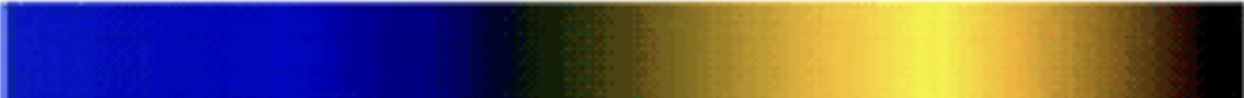
\includegraphics[width=.7\columnwidth,height=.9\baselineskip]{Figures/01_P.png}}$ \\
        D型色覚 & $\vcenter{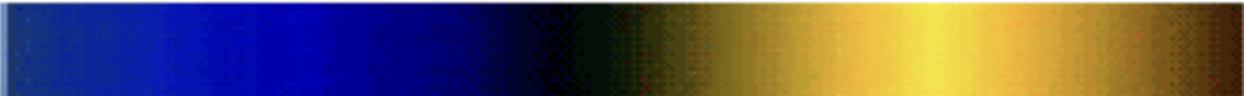
\includegraphics[width=.7\columnwidth,height=.9\baselineskip]{Figures/02_D.png}}$ \\
        T型色覚 & $\vcenter{
\includegraphics[width=.7\columnwidth,height=.9\baselineskip]{Figures/03_T.png}}$ \\
        \hline
    \end{tabularx}
\end{table}
\tblref{tbl:各色覚の見え方}より,4種の色覚に対応する色を決定する.
この実験では,講義一覧,折れ線グラフ,円グラフを4つの色覚に対応できるように設計する.
各コンテンツに対して,各色覚での見え方を結果として出力する.出力には,ImageJアプリケーションのVischeckJ1プラグインを利用する.
VischeckJ1は,イメージに対して,P型,D型,T型色覚での見え方を表示するプラグインである.\\
\kadai{講義一覧}\par
HTMLの\texttt{table}タグを用いて,講義一覧を作成する.各講義の「専門基礎科目」,「専門発展科目」,「専門領域科目」の背景色と,履修登録必須科目の文字色を,CSSで設定する.
デフォルトのセル背景配色を\tblref{tbl:デフォルト配色}に示す.
また,履修登録必須科目は,\texttt{<p1></p1>}タグ内の\texttt{color}属性で指定し,色を\rulebox{[HTML]{ff0000}}{\#ff0000}とする.
\begin{table}[H]
    \centering
    \caption{デフォルト配色}
    \label{tbl:デフォルト配色}
    \begin{tabularx}{\columnwidth}{RRR}
        \multicolumn{1}{c}{分類} & \multicolumn{1}{c}{セル背景色}          & \multicolumn{1}{c}{\texttt{class}名} \\
        \hline
        専門基礎科目                 & \rulebox{[HTML]{55bb55}}{\#55bb55} & \texttt{kiso}                       \\
        専門発展科目                 & \rulebox{[HTML]{ff9900}}{\#ff9900} & \texttt{hatten}                     \\
        専門領域科目                 & \rulebox{[HTML]{66aaaa}}{\#66aaaa} & \texttt{ryouiki}                    \\
        \hline
    \end{tabularx}
\end{table}
\begin{table}[H]
    \centering
    \caption{カラーユニバーサルデザイン配色}
    \label{tbl:CND配色}
    \begin{tabularx}{\columnwidth}{RRR}
        \multicolumn{1}{c}{分類} & \multicolumn{1}{c}{セル背景色}          & \multicolumn{1}{c}{\texttt{class}名} \\
        \hline
        専門基礎科目                 & \rulebox{[HTML]{B4EBFA}}{\#b4ebfa} & \texttt{kiso}                       \\
        専門発展科目                 & \rulebox{[HTML]{FFD1D1}}{\#ffd1d1} & \texttt{hatten}                     \\
        専門領域科目                 & \rulebox{[HTML]{FFFF99}}{\#ffff99} & \texttt{ryouiki}                    \\
        \hline
    \end{tabularx}
\end{table}
\rulebox{[HTML]{B4EBFA}}{\#b4ebfa}は,\rulebox{[HTML]{FFD1D1}}{\#ffd1d1},\rulebox{[HTML]{FFFF99}}{\#ffff99}は,RGB三原色を多く含んでいる.
この3色の組み合わせは,3原色の中で1つの認識が困難でも,ほかの2色で識別が可能である.
これらは白に近い淡い色であり,文字色を\rulebox{{black}}{black}にすることで,色覚によらず文字をはっきりと認識できる.
履修登録必須科目は,色に依存しないように文字色を変えず,\textbf{\underline{文字を太くし,下線を引く}}ことで表現した(\srcref{src:太字と下線を設定するCSS}).\\
\begin{lstlisting}[caption={太字と下線を設定するCSS},label={src:太字と下線を設定するCSS}]
p1 {
    font-weight: bold;
    text-decoration: underline;
}
\end{lstlisting}
\kadai{折れ線グラフ}\par
JavaScriptで記述された折れ線グラフを,カラーユニバーサルデザインに従って変更する.以下の点を変更する.
\begin{itemize}
    \item 背景の灰色グラデーションを削除する.
    \item 線の太さを太くする.
    \item マークの形状を商品別に変更する.
    \item 線の配色を変更する.
          \begin{itemize}
              \item \rulebox{[HTML]{0080FF}}{\#0080ff},\rulebox{[HTML]{BFBFBF}}{\#bfbfbf}は色覚によらず色が見える.
              \item \rulebox{[HTML]{FF0000}}{\#ff0000}はP型,D型色覚には異なった色に見えるが,ほかの2つと重複しない.
              \item 今回は,線自体が値を示すので,淡い色ではなく,濃い色を採用した.
          \end{itemize}
\end{itemize}
マーク形状,マークと線の太さ,背景色と線色の変更は\srcref{src:折れ線グラフの変更}で行う.
\begin{lstlisting}[caption={折れ線グラフの変更},label={src:折れ線グラフの変更},language={JavaScript}]
var parms = {
    // 略
    // 背景色の変更
    backgroundColor: "#ffffff", 
	gbackgroundColor: "#ffffff",
    lineWidth: 3, // ラインの太さ
    dotRadius: 4, // マークの太さ
    // マークの形状
    dotType: ["diamond", "square", "disc"],
    // 略
}
// 略
var colors = ["0,128,255", "255,0,0", "191,191,191"]; // 線色の設定
\end{lstlisting}
\kadai{円グラフ}\par
\begin{itemize}
    \item 円グラフの配色を変更する.以下の配色を,いずれの色覚でも似た色どうしが隣り合わないように配置する.
          \begin{itemize}
              \item \rulebox{[HTML]{FF0000}}{\#ff0000}
              \item \rulebox{[HTML]{4169FF}}{\#4169ff}
              \item \rulebox{[HTML]{FFFF00}}{\#ffff00}
              \item \rulebox{[HTML]{00FFFF}}{\#00ffff}
          \end{itemize}
\end{itemize}
円グラフの配色を変更は\srcref{src:円グラフの変更}で行う.
\begin{lstlisting}[caption={円グラフの変更},label={src:円グラフの変更},language={JavaScript}]
var colors = ["255,0,0", "65,105,255", "255,255,0", "0,255,255"]; // 円色の変更
\end{lstlisting}